
\subsection{Analyse Eventim}
Die Eventim Startseite und ihre Unterseiten, wie die Veranstaltungsseite, wurden untersucht. Dabei trat ein verletztes Kriterium vermehrt auf. Das Kriterium 1.4.3 "Mindestkontrast" wurde so oft verletzt wie auf keiner anderen Website. Es sind also nicht nur einzelne Elemente betroffen, sondern bei der gesamten Gestaltung wurden die Kontrastverhältnisse nicht mit beachtet.

\begin{figure}[H]
    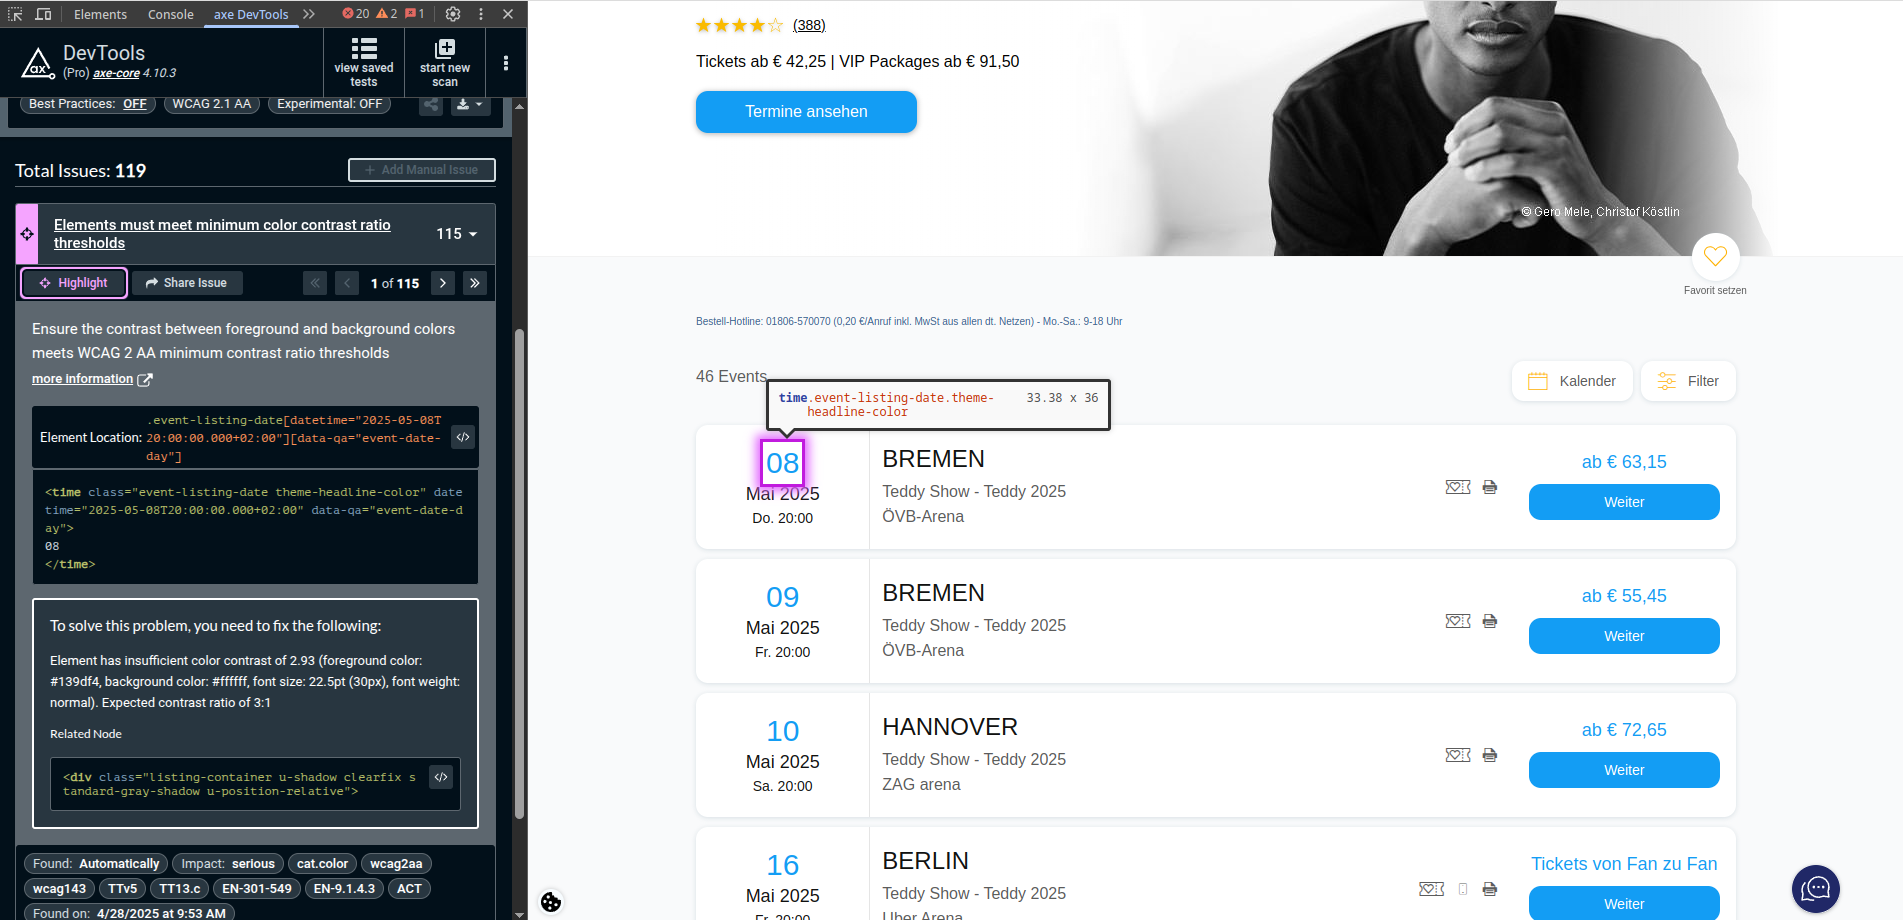
\includegraphics[width=\textwidth]{img/eventim_failed_minimum-contrast.png}
    \caption{Kontrastprobleme auf der Startseite}
\end{figure}

Zusätzlich wurden auch bei den Social-Media-Links keine Labels angegeben. 

\begin{figure}[H]
    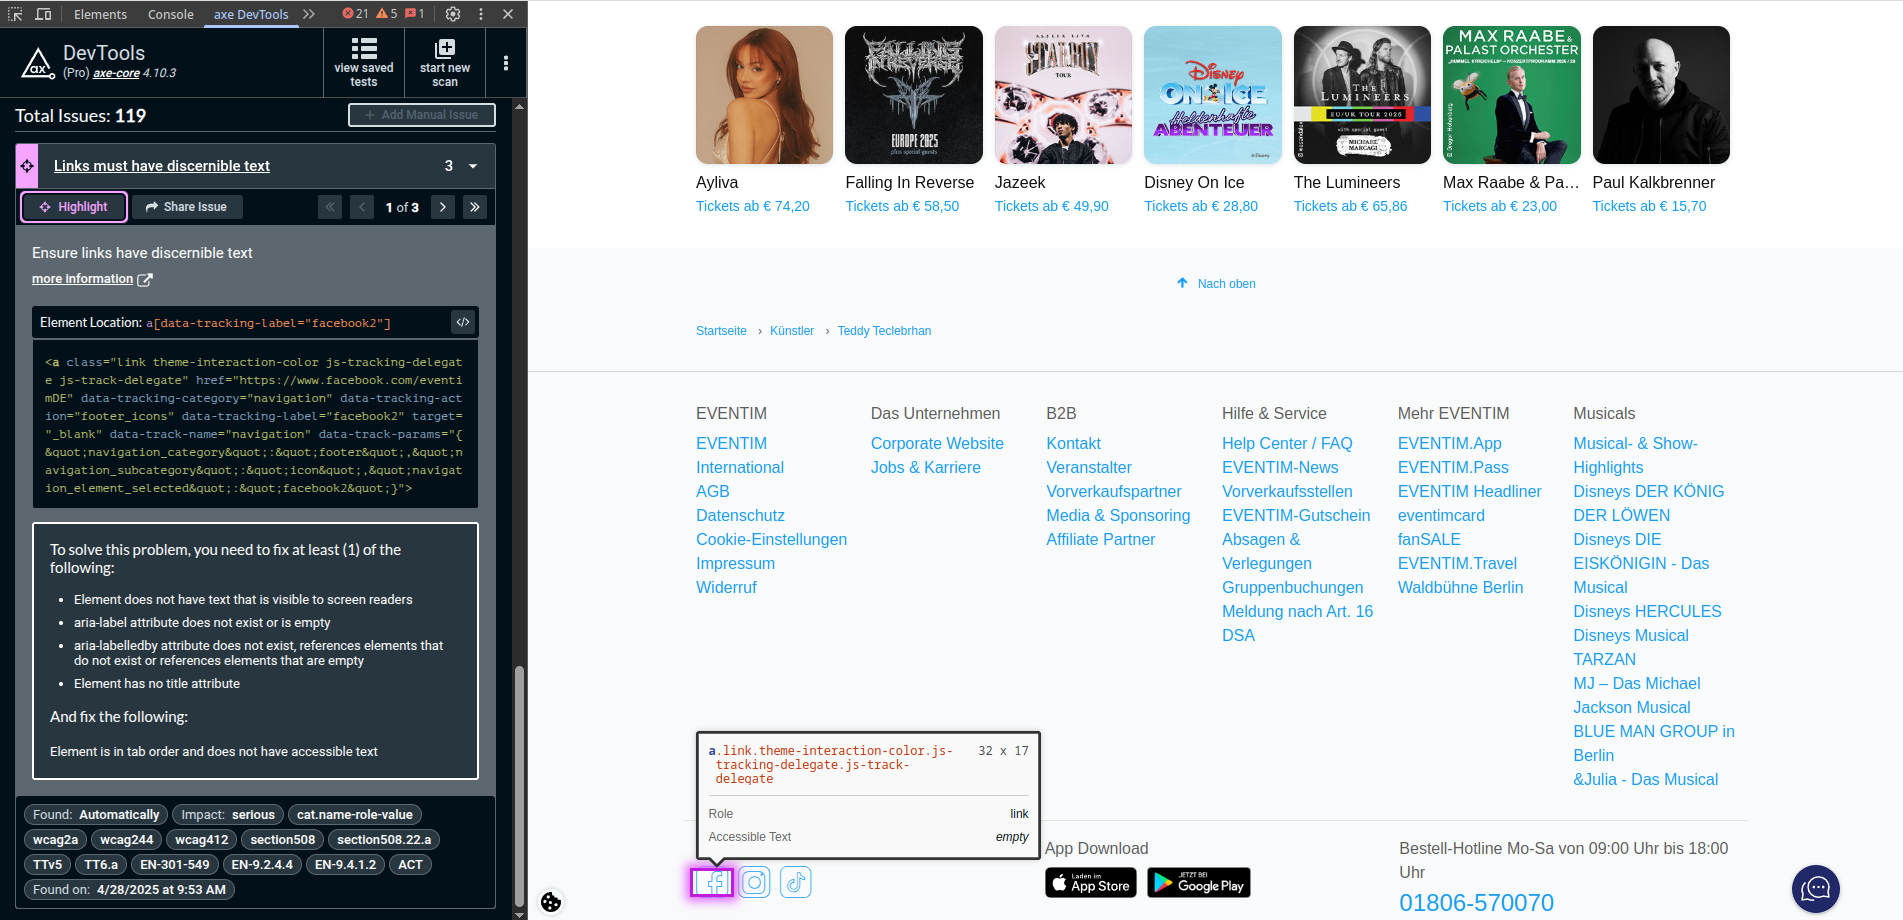
\includegraphics[width=\textwidth]{img/eventim_social-links-no-accessible-text.png}
    \caption{Fehlendes Label bei einem Link}
\end{figure}

Und wie beim VBB auch, wurde kein zugänglicher Name für den iframe angegeben. Das ist ein Verstoß gegen Kriterium 4.1.2 "Name, Rolle, Wert".
\begin{figure}[H]
    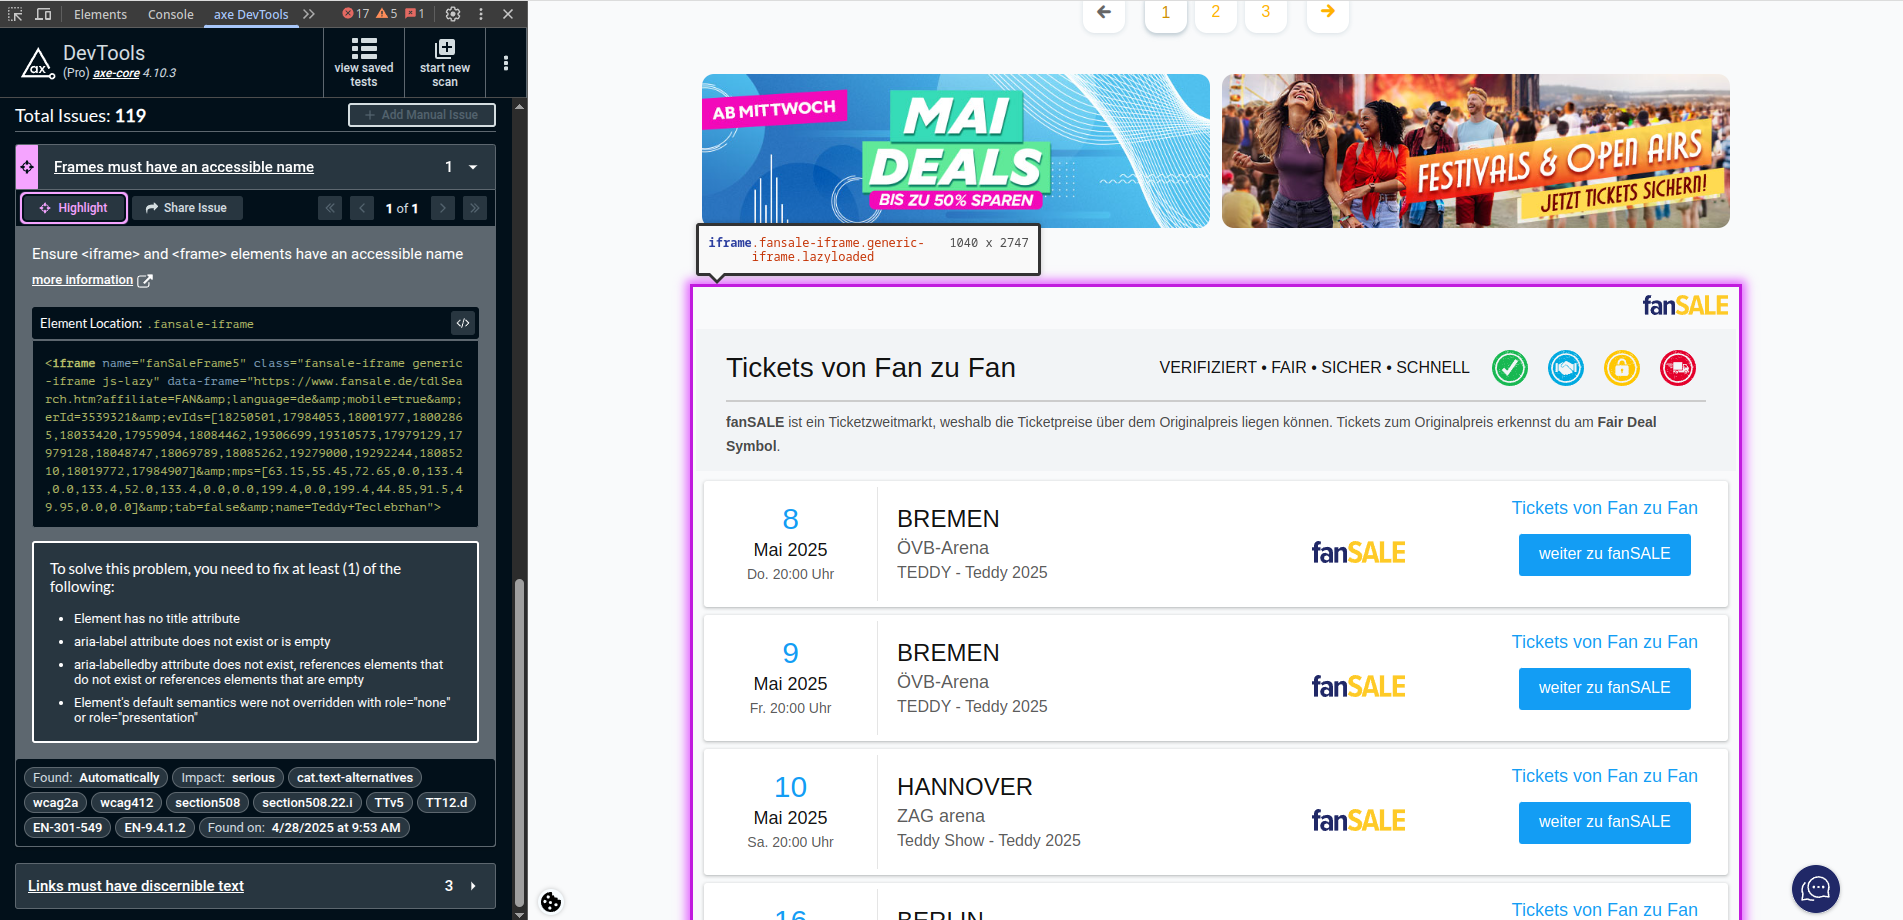
\includegraphics[width=\textwidth]{img/eventim_iframe-no-alt-text.png}
    \caption{Fehlendes Label bei einem Link}
\end{figure} 

Bei der Betrachtung der gesamten Zahlen fällt der Schwerpunkt der verletzten Kriterien deutlich auf. Die Kontraste wurden in der Gestaltung nicht berücksichtigt und sind damit auch auf der gesamten Seite zu finden. Auch die Social-Media-Links sind auf jeder Seite vorhanden. 

\begin{figure}[H]
\begin{tikzpicture}
\begin{axis}[
    width=\textwidth,
    height=10cm,
    ybar,
    bar width=12pt,
    xlabel={WCAG-Kriterium},
    ylabel={Fehleranzahl},
    symbolic x coords={ 9.1.3.1, 9.1.4.3, 9.2.4.1, 9.2.4.4, 9.4.1.2 },
    xtick=data,
    x tick label style={rotate=45, anchor=east},
    ymin=0,
    ymax=350,
    enlarge x limits=0.1,
    legend style={cells={anchor=west}, legend pos=north east},
    nodes near coords,
    nodes near coords style={font=\scriptsize},
]
\addplot table[x=WCAG-Kriterium,y=Fehleranzahl_axe,col sep=tab]{csv/output/wcag_analyse_Eventim_xxxx.csv};
\addplot table[x=WCAG-Kriterium,y=Fehleranzahl_WAVE,col sep=tab]{csv/output/wcag_analyse_Eventim_xxxx.csv};
\legend{axe,WAVE}
\end{axis}
\end{tikzpicture}
\caption{Auswertung Analyse Eventim}
\end{figure}
